\documentclass{beamer}
%Imports and customization
\usepackage{tikz}
\usepackage{graphicx}
\usepackage{tikz-feynman}
\usepackage{ulem}
\usepackage{colortbl}
\graphicspath{ 
    {./images/}
}

\beamertemplatenavigationsymbolsempty
\setbeamertemplate{sidebar right}{}
\setbeamertemplate{footline}{
    \hfill\usebeamertemplate***{navigation symbols}
    \hspace{1cm}\insertframenumber{}/\inserttotalframenumber
}
\setbeamertemplate{caption}{\raggedright\insertcaption\par}
\setbeamersize{text margin left=4mm,text margin right=4mm} 

\setbeamerfont{itemize/enumerate body}{size=\scriptsize}
\setbeamerfont{itemize/enumerate subbody}{size=\scriptsize}
\setbeamerfont{itemize/enumerate subsubbody}{size=\scriptsize}


%Custom Macros
\newcommand{\statwarn}{
    \tiny \color{red} Absolute numbers here mean NOTHING. Plots are based on small (100k events) samples, and are highly biased. All that matters is relative position!
}


% WARNING: When using these commands, the image argument must
% NOT have spaces between itself and the braces
\newcommand{\fullscreenimage}[2]{
    \frame{
        \frametitle{#1} 
        \begin{figure}
        \includegraphics[height=0.9\textheight,width=\textwidth,keepaspectratio]{#2}
        \end{figure}
    }
}


\newcommand{\importpdf}[3]{
    \frame{
        \begin{columns}\column{\dimexpr\paperwidth-10pt}
        \begin{figure}
        \includegraphics[page=#2,height=0.8\textheight,width=\textwidth,keepaspectratio]{#1}
        \end{figure}

        {\tiny #3}
        \end{columns}
    }
}


\newcommand{\displayone}[3]{
    \frame{
        \frametitle{#1} 
        \begin{columns}
            \begin{column}{0.5\textwidth}
                #2
            \end{column}
            \begin{column}{0.5\textwidth}
                \begin{figure}
                    \includegraphics[width=\linewidth,height=\textheight,keepaspectratio]{#3}
                \end{figure}
            \end{column}
        \end{columns}
    }
}

\newcommand{\displayonelarge}[3]{
    \frame{
        \frametitle{#1} 
        \begin{columns}
            \begin{column}{0.3\textwidth}
                #2
            \end{column}
            \begin{column}{0.7\textwidth}
                \begin{figure}
                    \includegraphics[width=\linewidth,height=0.8\textheight,keepaspectratio]{#3}
                \end{figure}
            \end{column}
        \end{columns}
    }
}


\newcommand{\displaytwo}[4]{
    \frame{
        \frametitle{#1} 
        #2
        \begin{columns}
            \begin{column}{0.5\textwidth}
                \begin{figure}
                    \includegraphics[width=\linewidth,height=\textheight,keepaspectratio]{#3}
                \end{figure}
            \end{column}
            \begin{column}{0.5\textwidth}
                \begin{figure}
                    \includegraphics[width=\linewidth,height=\textheight,keepaspectratio]{#4}
                \end{figure}
            \end{column}
        \end{columns}
    }
}

\newcommand{\displaytwocaption}[6]{
    \frame{
        \frametitle{#1} 
        #2
        \begin{columns}
            \begin{column}{0.5\textwidth}
                \begin{figure}
                    \includegraphics[width=\linewidth,height=\textheight,keepaspectratio]{#3}
                    \caption{#4}
                \end{figure}
            \end{column}
            \begin{column}{0.5\textwidth}
                \begin{figure}
                    \includegraphics[width=\linewidth,height=\textheight,keepaspectratio]{#5}
                    \caption{#6}
                \end{figure}
            \end{column}
        \end{columns}
    }
}

\newcommand{\displaytwoVcaption}[6]{
    \frame{
        \begin{columns}
            \begin{column}{0.5\textwidth}
                \frametitle{#1} 
                #2
            \end{column}
            \begin{column}{0.5\textwidth}
                \begin{figure}
                    \includegraphics[width=\linewidth,height=0.3\textheight,keepaspectratio]{#3}
                    \caption{#4}
                \end{figure}

                \begin{figure}
                    \includegraphics[width=\linewidth,height=0.3\textheight,keepaspectratio]{#5}
                    \caption{#6}
                \end{figure}
            \end{column}
        \end{columns}
    }
}


\newcommand{\displaythree}[5]{
    \frame{
        \begin{columns}[T]
            \begin{column}{0.4\textwidth}
                {\usebeamercolor[fg]{title} \insertframetitle{#1} }\\
                \vspace{5mm}
                #2
            \end{column}
            \begin{column}{0.4\textwidth}
                \begin{figure}
                    \includegraphics[width=\linewidth,height=\textheight,keepaspectratio]{#3}
                \end{figure}
            \end{column}
        \end{columns}
        \begin{columns}[T]
            \begin{column}{0.4\textwidth}
                \begin{figure}
                    \includegraphics[width=\linewidth,height=\textheight,keepaspectratio]{#4}
                \end{figure}
            \end{column}
            \begin{column}{0.4\textwidth}
                \begin{figure}
                    \includegraphics[width=\linewidth,height=\textheight,keepaspectratio]{#5}
                \end{figure}
            \end{column}
        \end{columns}
    }
}


\newcommand{\displayfour}[5]{
    \frame{
        \frametitle{#1} 
        \begin{columns}[T]
            \begin{column}{0.4\textwidth}
                \begin{figure}
                    \includegraphics[width=\linewidth,height=\textheight,keepaspectratio]{#2}
                \end{figure}
            \end{column}
            \begin{column}{0.4\textwidth}
                \begin{figure}
                    \includegraphics[width=\linewidth,height=\textheight,keepaspectratio]{#3}
                \end{figure}
            \end{column}
        \end{columns}
        \begin{columns}[T]
            \begin{column}{0.4\textwidth}
                \begin{figure}
                    \includegraphics[width=\linewidth,height=\textheight,keepaspectratio]{#4}
                \end{figure}
            \end{column}
            \begin{column}{0.4\textwidth}
                \begin{figure}
                    \includegraphics[width=\linewidth,height=\textheight,keepaspectratio]{#5}
                \end{figure}
            \end{column}
        \end{columns}
    }
}


\newcommand{\pstrike}[2]{
    \only<-\the\numexpr#1-1>{#2}
    \only<#1->{\sout{#2}}
}


\newcommand{\announcesection}[1]{
    \section{#1}
    \frame{
        \begin{center}
            {\huge #1} 
        \end{center}
    }
}

\newcommand{\kvv}{\kappa_{2V}}
\newcommand{\kl}{\kappa_{\lambda}}
\newcommand{\kv}{\kappa_{V}}

\newcommand{\fkvv}[1]{\kappa_{2V,#1}}
\newcommand{\fkl} [1]{\kappa_{\lambda,#1}}
\newcommand{\fkv} [1]{\kappa_{V,#1}}

\newcommand{\importpdfwpages}[3]{
    \foreach \pageN in {#2,...,#3}{
        \importpdf{#1}{\pageN}{}
    }
}

\newcommand{\hyper}[2]{{\color{blue}\href{#1}{#2}}}



%Begin Presentation
\begin{document}
\setbeamercolor{background canvas}{bg=}
\title{
    Improved Constraints on \\the Standard Model Higgs Self-Interaction \\
    Using a Search for \hhbbbb \\via the Vector-Boson Fusion Production Mode \\
    at $\sqrt{s}=13~\mathrm{TeV}$ in 126 \ifb of Data \\Collected by the ATLAS Experiment
}
\subtitle{\vspace{3mm}Ph.D. Dissertation Defense}

\author{Chris Milke\\{\small Committee Members:\\Stephen Sekula, Chris Pollard, Roberto Vega, Jingbo Ye}}
\institute{Southern Methodist University}
\date{6 July, 2022}

\frame{\titlepage}
\title{
    Smashy Physics!\\Gaining a Better Understanding of the Smashing\\Using Smashy Math
}
\frame{\titlepage}
\frame{\frametitle{Overview} \tableofcontents}
%\announcesection{Introduction}

% Theory 1: SM
\displayonelarge{The Standard Model of Particle Physics}{
    {\footnotesize
    Description of all (known) matter.
    \vspace{5mm}

    Founded on paradigm (symmetry) which relied on
        principle that ``forces'' can be described
        as interactions mediated by \textit{massless} gauge boson particles.
    \vspace{5mm}

    Confoundingly, the W and Z bosons \textit{do} have mass.
    The cornerstone of the SM is in how it resolves this mass...
        %requiring either a modification to 
        %(or complete overhaul of) the theory.}
    }
}{theory/Standard_Model_of_Elementary_Particles}

% Theory 2: Higgs Field
\displayone{The Higgs Mechanism}{
    The Higgs mechanism posits the existence of a ``Higgs Field''
        which induces mass in any particles it interacts with it.
    \vspace{5mm}

    This field was predicted to manifest in the form of a scalar particle,
        the Higgs boson,
        and was detected in 2012 by the CMS and ATLAS experiments.
    \vspace{5mm}
}{theory/higgspotential}

% VVh, VVHH, HHH, HHHH (backup)
\frame{
    \frametitle{Electroweak-Higgs Interactions}

    Some key properties of the Higgs are still poorly understood,
        but could be probed via di-Higgs production.


    \begin{figure}
    \centering
    \begin{subfigure}{0.32\textwidth} 
        \resizebox{0.9\textwidth}{!}{
\begin{tikzpicture} \begin{feynman}
    \vertex (kv) {$\kv$};
    \vertex [right=of kv] (h) {$h$};
    \vertex [above left=of kv] (vb1) {$V_1$};
    \vertex [below left=of kv] (vb2) {$V_2$};

    \diagram* {
        (vb1) -- [boson] (kv) -- [boson] (vb2),
        (kv) -- [scalar] (h),
    };
\end{feynman} \end{tikzpicture}
}
 
        \caption{$VVh$}
    \end{subfigure}
    \begin{subfigure}{0.32\textwidth}
        \resizebox{0.8\textwidth}{!}{
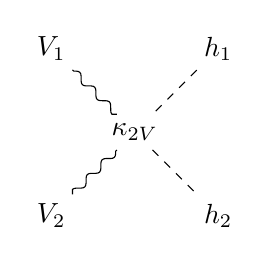
\begin{tikzpicture} \begin{feynman}
    \vertex (k2v) {$\kvv$};
    \vertex [above right=of k2v] (h1) {$h_1$};
    \vertex [below right=of k2v] (h2) {$h_2$};
    \vertex [above left=of k2v] (vb1) {$V_1$};
    \vertex [below left=of k2v] (vb2) {$V_2$};

    \diagram* {
        (vb1) -- [boson] (k2v) -- [boson] (vb2),
        (h1) -- [scalar] (k2v) -- [scalar] (h2),
    };
\end{feynman} \end{tikzpicture}
}
 
        \caption{$VVhh$}
    \end{subfigure}
    \begin{subfigure}{0.32\textwidth}
        \resizebox{0.9\textwidth}{!}{
\begin{tikzpicture} \begin{feynman}
    \vertex (h0) {$h_0$};
    \vertex [right=of h0] (kl) {$\kl$};
    \vertex [above right=of kl] (h1) {$h_1$};
    \vertex [below right=of kl] (h2) {$h_2$};

    \diagram* {
        (h0) -- [scalar] (kl),
        (h1) -- [scalar] (kl) -- [scalar] (h2),
    };
\end{feynman} \end{tikzpicture}
}
 
        \caption{$hhh$}
    \end{subfigure}
    \end{figure}

    The Standard Model predicts how frequently these interactions should occur.
    By providing the conditions necessary for these interactions,
        one can measure how often they actually occur vs their theoretically predicted rate
        (the interactions' ``$kappa$-value'').
}

%% Theory 3: Higgs Lagrangian and its (electroweak) couplings
%\frame{
%    \frametitle{}
%    {\footnotesize
%    \begin{equation} \begin{split} \label{eq:higgskappas}
%        \Lag_h &= \frac{1}{2} \left(\partial^2 - m_h^2 \right) h^2
%            + \kv g_{HVV} V^2 h + \kvv \frac{g_{HHVV}}{2} V^2 h^2
%            + \kl \frac{g_{HHH}}{3!} h^3 + \kappa_{2\lambda} \frac{g_{HHHH}}{4!} h^4
%         \nonumber
%    \end{split} \end{equation}
%    }
%}

% Theory 3: di-Higgs and VBF->HH->bbbb
\frame{
    \frametitle{Vector Boson Fusion, di-Higgs Production, and the All-Hadronic Final State}
    \begin{columns}
        \begin{column}{0.4\textwidth}
            \resizebox{.8\textwidth}{!}{
\begin{tikzpicture} \begin{feynman}
    \vertex (c2v) {???};
    \vertex [above right=of c2v] (h1) {$h_1$};
    \vertex [below right=of c2v] (h2) {$h_2$};
    \vertex [above left=of c2v] (vb1);
    \vertex [below left=of c2v] (vb2);
    \vertex [left=of vb1] (q1) {$q_1$};
    \vertex [left=of vb2] (q2) {$q_2$};
    \vertex [above right=of h1] (b1) {$b$};
    \vertex [below right=of h2] (bbar2) {$\bar b$};
    \vertex [below=of b1] (bbar1) {$\bar b$};
    \vertex [above=of bbar2] (b2) {$b$};

    \vertex [above=of b1] (q3) {$q_3$};
    \vertex [below=of bbar2] (q4) {$q_4$};

    \diagram* {
        (q1) -- (vb1) -- (q3),
        (q2) -- (vb2) -- (q4), 
        (vb1) -- [boson] (c2v) -- [boson] (vb2),
        (h1) -- [scalar] (c2v) -- [scalar] (h2),
        (b1) -- (h1) -- (bbar1),
        (b2) -- (h2) -- (bbar2),
    };
\end{feynman} \end{tikzpicture}
}
 
        \end{column}
        \begin{column}{0.6\textwidth}
            \begin{table}
\centering
\scriptsize
\begin{tabular}{|l|l|l|}
    \hline
    Decay channel & Branching ratio & Rel. uncertainty  \\
    \hline
    $ H \to b \bar{b}        $    & $5.82 \times 10^{-1} $    & $ +1.2\% \atop -1.3\% $ \\
    $ H \to W^+ W^-          $    & $2.14 \times 10^{-1} $    & $\pm 1.5\%        $   \\
    $ H \to \tau^+ \tau^-    $    & $6.27 \times 10^{-2} $    & $\pm 1.6\%        $   \\
    $ H \to c \bar{c}        $    & $2.89 \times 10^{-2} $    & $ +5.5\% \atop -2.0\% $ \\
    $ H \to ZZ               $    & $2.62 \times 10^{-2} $    & $\pm 1.5\%        $   \\
    $ H \to \gamma \gamma    $    & $2.27 \times 10^{-3} $    & $    2.1\%        $   \\
    $ H \to Z \gamma         $    & $1.53 \times 10^{-3} $    & $\pm 5.8\%        $  \\
    $ H \to \mu^+ \mu^-      $    & $2.18 \times 10^{-4} $    & $\pm 1.7\%        $  \\
    \hline
\end{tabular}
\end{table}

        \end{column}
    \end{columns}
}


\frame{
    \frametitle{\hhproc Production}

    \begin{figure}
    \centering
    \begin{subfigure}{0.32\textwidth} 
        \resizebox{0.9\textwidth}{!}{
\begin{tikzpicture} \begin{feynman}
    \vertex (kv1) {$\kv$};
    \vertex [below=of kv1] (kv2) {$\kv$};
    \vertex [right=of kv1] (h1) {$h_1$};
    \vertex [right=of kv2] (h2) {$h_2$};
    \vertex [above left=of kv1] (vb1);
    \vertex [below left=of kv2] (vb2);
    \vertex [left=of vb1] (q1) {$q_{1}$};
    \vertex [left=of vb2] (q2) {$q_{2}$};

    \vertex [above=of h1] (q3) {$q_{3}$};
    \vertex [below=of h2] (q4) {$q_{4}$};

    \diagram* {
        (q1) -- (vb1) -- (q3),
        (q2) -- (vb2) -- (q4), 
        (vb1) -- [boson] (kv1) -- [boson] (kv2)-- [boson] (vb2),
        (h1) -- [scalar] (kv1),
        (h2) -- [scalar] (kv2),
    };
\end{feynman} \end{tikzpicture}
}
 
        \caption{$M_t$}
        \label{fig:tree_level_vbfhh:kv}
    \end{subfigure}
    \begin{subfigure}{0.32\textwidth}
        \resizebox{0.9\textwidth}{!}{
\begin{tikzpicture} \begin{feynman}
    \vertex (kv) {$\kv$};
    \vertex [right=of kv] (kl) {$\kl$};
    \vertex [above right=of kl] (h1) {$h_1$};
    \vertex [below right=of kl] (h2) {$h_2$};
    \vertex [above left=of kv] (vb1);
    \vertex [below left=of kv] (vb2);
    \vertex [left=of vb1] (q1) {$q_{1}$};
    \vertex [left=of vb2] (q2) {$q_{2}$};

    \vertex [above=of h1] (q3) {$q_{3}$};
    \vertex [below=of h2] (q4) {$q_{4}$};

    \diagram* {
        (q1) -- (vb1) -- (q3),
        (q2) -- (vb2) -- (q4), 
        (vb1) -- [boson] (kv) -- [boson] (vb2),
        (kv) -- [scalar] (kl),
        (h1) -- [scalar] (kl) -- [scalar] (h2),
    };
\end{feynman} \end{tikzpicture}
}
 
        \caption{$M_s$}
        \label{fig:tree_level_vbfhh:kl}
    \end{subfigure}
    \begin{subfigure}{0.32\textwidth}
        \resizebox{0.8\textwidth}{!}{
\begin{tikzpicture} \begin{feynman}
    \vertex (k2v) {$\kvv$};
    \vertex [above right=of k2v] (h1) {$h_1$};
    \vertex [below right=of k2v] (h2) {$h_2$};
    \vertex [above left=of k2v] (vb1);
    \vertex [below left=of k2v] (vb2);
    \vertex [left=of vb1] (q1) {$q_{1}$};
    \vertex [left=of vb2] (q2) {$q_{2}$};

    \vertex [above=of h1] (q3) {$q_{3}$};
    \vertex [below=of h2] (q4) {$q_{4}$};

    \diagram* {
        (q1) -- (vb1) -- (q3),
        (q2) -- (vb2) -- (q4), 
        (vb1) -- [boson] (k2v) -- [boson] (vb2),
        (h1) -- [scalar] (k2v) -- [scalar] (h2),
    };
\end{feynman} \end{tikzpicture}
}
 
        \caption{$M_x$}
        \label{fig:tree_level_vbfhh:k2v}
    \end{subfigure}
    \end{figure}

    \begin{equation} \begin{split}
        \sigma &\propto |  \kv^2 M_t + \kv \kl M_s + \kvv M_x |^2 \\
        \sigma &\propto \kv^2 \kl^2 a_1 + \kv^4 a_2 + \kvv^2 a_3 + \kv^3 \kl a_4 + \kv \kl \kvv a_5 + \kv^2 \kvv a_6
    \end{split} \end{equation}
}

% LHC 1: xsec/lumi
\frame{
    \frametitle{Cross-section and Integrated Luminosity}

    {
    \begin{equation} \begin{split}
        \textrm{Expected Events} &= (\textrm{Probability}) \times (\textrm{Number of repeated trials}) \\
        &\downarrow \\
        \textrm{Expected Events} &= \sigma \times L_{\textrm{integrated}}
        \nonumber
    \end{split} \end{equation}
    }
    \vspace{5mm}

    \begin{center}
    \begin{tabular}{ rll }
    $\sigma$ & $\rightarrow$ & Units of cross-sectional area (femto-barns, $fb = 10^{-43} m^2$);\\
        &&Purely a function of theory\\
    \\
    $L_{\textrm{integrated}}$ & $\rightarrow$ & Units of inverse area ($\ifb$);\\
        && Purely a function of experimental setup 
    \end{tabular}
    \end{center}


}

%\displayone{Cross-section and Luminosity}{
%    {\scriptsize
%    \begin{equation} \begin{split}
%        %\frac{\mathcal{P}_{\textrm{hit}}}{\textrm{throw}} &= \frac{\textrm{Area}_{\textrm{object}}}{\textrm{Area}_{\textrm{total}}} \\
%        %\textrm{expected hits} &= \frac{\mathcal{P}_{\textrm{hit}}}{{\textrm{throw}}} \times N_{\textrm{throws}}
%        %N_{\textrm{throws}} &= \frac{N_{\textrm{throws}}}{\Delta t} \times \Delta t \\
%        %\textrm{expected hits} &= \frac{\mathcal{P}_{\textrm{hit}}}{{\textrm{throw}}} \times N_{\textrm{throws}}
%        \frac{\mathcal{P}_{\textrm{hit}}}{\textrm{throw}} &= \frac{\xsec}{\textrm{Area}_{\textrm{total}}} \\
%        \frac{\textrm{expected hits}}{\Delta t} &= \frac{\mathcal{P}_{\textrm{hit}}}{{\textrm{throw}}} \times \frac{\textrm{throws}}{\textrm{\Delta t}} \\
%        \textrm{expected hits} &= \frac{\textrm{expected hits}}{\Delta t} \times {\Delta t}
%        \nonumber
%    \end{split} \end{equation}
%    \vspace{3mm}
%
%    \begin{equation} \begin{split}
%        \dXsec &\propto | M | ^2 \\
%        \xsec &= \int \dXsec d\Omega \\
%        L_{\textrm{instantaneous}} &= \frac{1}{\textrm{Area}_{\textrm{total}}} \times \frac{N_{\textrm{throws}}}{\Delta t} \\
%        L_{\textrm{integrated}} &= \int L_{\textrm{instantaneous}} dt \\
%        \textrm{expected events} &= \xsec \times L_{\textrm{integrated}}
%        \nonumber
%    \end{split} \end{equation}
%    }
%}{introduction/xsec_ball}

%\frame{
%    \frametitle{Cross-section and Luminosity}
%    \begin{columns}
%        \begin{column}{0.4\textwidth}
%        \end{column}
%        \begin{column}{0.6\textwidth}
%
%        \end{column}
%    \end{columns}
%}

% LHC 1: overview
\displaytwoV{The Large Hadron Collider}{
    \vspace{10mm}
    \begin{itemize}
        \item Constructed 1995-2007
        \item On border of Switzerland and France
        \item 50-175 meters underground
        \item 26.7 km radius 
        \item 13 TeV center-of-mass collision energy
        \item 139 \ifb of data delivered to Point 1 (126 are used for my analysis)
    \end{itemize}
}{introduction/lhc}{introduction/lhc_pipe}


% ATLAS 1: overview
\displayonelarge{The ATLAS Experiment}{
    {\small
    Massive particle detector array,
        forming a high hermetic, (nearly) $4\pi$ 3D ``camera'' around the particle interaction region
    \vspace{8mm}

    Different subsytems have different roles:
    \begin{itemize}
        \item Tracker = momentum of charged particles
        \item Calorimeter = energy
        \item Muon System = N/A
    \end{itemize}
    }
}{atlas/atlas_xsec}

\announcesection{Data Processing}

% Tracks
\displayonelarge{Tracking}{
    {\footnotesize
        2T solenoid magnet bends charged particles traversing trackers.
        Helical trajectory is used to calculated particle momentum/mass/charge.
    }
}{processing/IDbriefing_figure1}

% Jets
\displayonelarge{Jets}{
    {\footnotesize
        Determines energy of particles by seeing how many plates of metal they can go through.
        E-Cal for electrons/photons,
            H-Cal for hadronic particles.

    }
}{reconstruction/ATLAS_Detector_Schematic_black_particles}

% Flavor Tagging
\displayone{Flavor Tagging}{
    Uses a recurrent Deep Learning neural net (DL1r) to distinguish b-jets from light-jets.
    Primarily takes advantage of secondary vertexing and impact parameter jet properties
}{reconstruction/dl1_performance_ljet}

% Selection
\frame{
    \frametitle{Event Selection}
    \begin{columns} \begin{column}{0.39\textwidth}
        {\tiny
        \begin{itemize}
            \item At least six jets total
            \begin{itemize}
                \item Central Jets: $|\eta| < 2.5$, $p_T > 40$ GeV
                \item Forward Jets: $2.5 < |\eta| \leq 4.5$, $p_T > 30$ GeV
            \end{itemize}
            \item Two \textit{anti}-b-tagged jets
            \begin{itemize}
                \item $ |\Delta \eta_{jj}| > 3.0 $,
                \item $M_{jj} > 1000$ GeV, and
                \item $p_{T,jj} < 65 $ GeV
            \end{itemize}
            \item At least 4 central, b-tagged jets
            \begin{itemize}
                \item $p_T > 40$ GeV
                \item paired up as reconstructed HH
                \item $ |\Delta \eta_{HH}| < 1.5 $
            \end{itemize}
            \item Using b-jet trigger DL1r 77\% working point,
                light jet acceptance of 0.59\%
        \end{itemize}
        }
    \end{column} \begin{column}{0.6\textwidth}
        \begin{figure}
            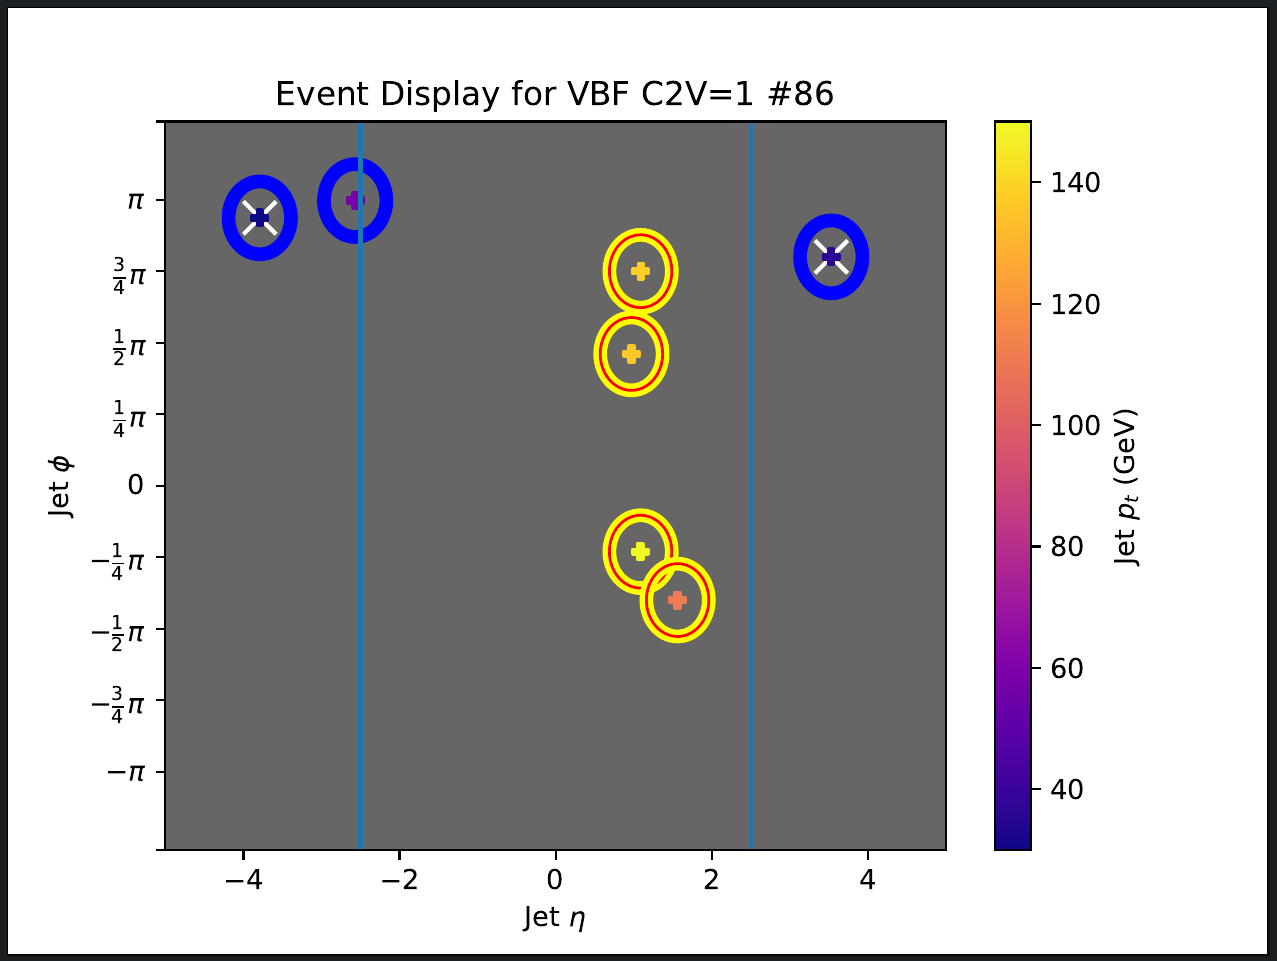
\includegraphics[width=\linewidth,height=0.9\textheight,keepaspectratio]{selection/event_display}
            \caption{\tiny Rings indicate jets;
                Yellow ring => b-tagged;
                Blue ring w/ white cross => VBF initial-scatter jets;
                ``+'' in center of rings => $p_T$;
                vertical lines denote "forward" vs "central" region.}
        \end{figure}
    \end{column} \end{columns}
}

% Background Events
\displaytwo{Data-driven Background Estimate}{
    \footnotesize{
        Multi-jet events (and some $\ttbar$ events) are a massive background.

        Can use data in which only 2 jets are b-tagged
            and massplane ``control regions'' to estimate background present in signal region.
    }
    \vspace{5mm}

    \begin{center}
    $ \textrm{Bgd}(4b, \textrm{Signal}) \approx 
         \textrm{Bgd}(4b, \textrm{Control}) \times \frac{
         \textrm{Bgd}(2b, \textrm{Signal}) }{
         \textrm{Bgd}(2b, \textrm{Control})} $
     \end{center}
    
    %Posit that 2b-tagged events are kinematically similar to 4b-tagged background.

}{selection/massplane_sig_all_4b_vbf_Xwt_1p5_k2V_0}
{background/massplane_dat_all_2b_vbf_Xwt_1.5}

\displayone{Background Reweighting}{
    {\footnotesize
        Kinematic differences exist between 2b and 4b;
             requires event-by-event reweighting

        \begin{center} 
        Example event:
        \vspace{3mm}

        \resizebox{0.3\textheight}{!}{ \begin{tabular}{ |l|r| }
            \hline
                $p_{T,H1}$ & 80 GeV \\ \hline
                $p_{T,H2}$ & 75 GeV \\ \hline
                $m_{HH}$ & 500 GeV \\ \hline
                $m_{jj}$ & 1200 GeV \\ \hline
                $\deta_{HH}$ & 1.1 \\ \hline
                \textbf{2b} rate & 8\% \\ \hline
                \textbf{4b} rate & 5\% \\ \hline
        \end{tabular}}
        \vspace{5mm}

            $\therefore$ reweight such an event by factor of 5/8
        \end{center}
        \vspace{3mm}
    }
}{background/crypto-mean-stdBS-m-hh-Control-Region-1-no-rw-all-4binclusive}

\displayfour{Reweighting Performance}
{background/crypto-mean-stdBS-m-hh-Control-Region-1-no-rw-all-4binclusive}
{background/crypto-mean-stdBS-m-hh-Control-Region-1-NN-all-4binclusive}
{background/crypto-mean-stdBS-dEta-hh-Control-Region-1-no-rw-all-4binclusive}
{background/crypto-mean-stdBS-dEta-hh-Control-Region-1-NN-all-4binclusive}

%{background/crypto-mean-stdBS-X-wt-tag-Control-Region-1-no-rw-all-4binclusive}
%{background/crypto-mean-stdBS-X-wt-tag-Control-Region-1-NN-all-4binclusive}

%\announcesection{Signal Modelling}

\displaytwo{Signal MC}{
    Different values for the $\kappa$'s (\kvv, \kl, \kv) leads to very different kinematic distributions and event yeilds.
    \vspace{5mm}

    We need large coverage of the 3-coupling parameter space, but signal samples are computationally expensive to produce.
}{signal/truth_lhe_HH_m}
%{signal/truth_lhe_jj_M}
{signal/truth_lhe_HH_dEta}


\newcommand{\lcm}[2]{
    #1_{#2}(
        m_{HH},
        m_{jj},
        ...
    )
}
\newcommand{\lcma}[1]{\lcm{a}{#1}}
\newcommand{\lcmb}[1]{\lcm{b}{#1}}

\frame{
    \frametitle{3D Coupling Dependence}
    {\footnotesize
        Some kind of shortcut is needed,
            but relationship between matrix element expansion and event yields
            is highly non-trivial due to distortion via acceptance/efficiency.

        \begin{equation} \begin{split}
            \sigma \propto \kv^2 \kl^2 a_1 + \kv^4 a_2 + \kvv^2 a_3 + \kv^3 \kl a_4 + \kv \kl \kvv a_5 + \kv^2 \kvv a_6
            \nonumber
        \end{split} \end{equation}
    }
    \begin{center}
    \resizebox{3mm}{!}{$\downarrow$}
    \end{center}
    {\footnotesize \begin{equation} \begin{alignedat}{3}
        & \frac{d^n \sigma}{d m_{HH} d m_{jj} d ...} = && &&\\
        \kv^2 \kl^2 &\times \lcma{1}
            + \qquad\:\: \kv^4 &&\times \lcma{2}
            + \quad\:\: \kvv^2 &&\times \lcma{3} \\
        + \kv^3 \kl &\times \lcma{4}
            + \kv \kl \kvv &&\times \lcma{5}
            + \kv^2 \kvv &&\times \lcma{5}
            \nonumber
    \end{alignedat} \end{equation} }
    \vspace{3mm}

    \begin{center}
    \resizebox{4mm}{!}{$\downarrow$}
    \begin{minipage}[b]{40mm}{\tiny
        hadronization, material interaction,\\
        reconstruction, selection
    }\end{minipage}
    \end{center}


    {\footnotesize \begin{equation} \begin{alignedat}{3}
        & \lcm{N}{\textrm{events}} = && && \\ 
        \kv^2 \kl^2 &\times \lcmb{1}
            + \qquad\:\: \kv^4 &&\times \lcmb{2}
            + \quad\:\: \kvv^2 &&\times \lcmb{3} \\
        + \kv^3 \kl &\times \lcmb{4}
            + \kv \kl \kvv &&\times \lcmb{5}
            + \kv^2 \kvv &&\times \lcmb{5}
            \nonumber
    \end{alignedat} \end{equation} }
}

% 6 variables, six equations, make a mess
\frame{
    \frametitle{6 Unknowns: Solve With 6 Equations}

    \vspace{5mm}

    \foreach \index in {1,2,3,4,5,6}{
        { \small $ N_\index
            = \fkv{\index}^2 \fkl{\index}^2 b_1
            + \fkv{\index}^4 b_2
            + \fkvv{\index}^2 b_3
            + \fkv{\index}^3 \fkl{\index} b_4
            + \fkv{\index} \fkl{\index} \fkvv{\index} b_5
            + \fkv{\index}^2 \fkvv{\index} b_6 $ }

        \vspace{5mm}
    }
}

% convert to matrix, show nice matrix solution
\frame{
    \frametitle{Linear Algebra Makes this Simple}

    \begin{columns}[T]
        \begin{column}{0.18\textwidth}
            $ \vec{N} = \begin{pmatrix} N_1 \\ N_2 \\ N_3 \\ N_4 \\ N_5 \\ N_6 \end{pmatrix} $
        \end{column}
        \begin{column}{0.15\textwidth}
            $ \vec{b} = \begin{pmatrix} b_1 \\ b_2 \\ b_3 \\ b_4 \\ b_5 \\ b_6 \end{pmatrix} $
        \end{column}
        \begin{column}{0.25\textwidth}
            $ \vec{f} = \begin{pmatrix} \kv^2 \kl^2 \\ \kv^4 \\ \kvv^2 \\ \kv^3 \kl \\ \kv \kl \kvv \\ \kv^2 \kvv \end{pmatrix} $
        \end{column}
        \begin{column}{0.4\textwidth}
            $ F = \begin{pmatrix}
                \vec{f}(\fkvv{1}, \fkl{1}, \fkv{1}) \\
                \vec{f}(\fkvv{2}, \fkl{2}, \fkv{2}) \\
                \vec{f}(\fkvv{3}, \fkl{3}, \fkv{3}) \\
                \vec{f}(\fkvv{4}, \fkl{4}, \fkv{4}) \\
                \vec{f}(\fkvv{5}, \fkl{5}, \fkv{5}) \\
                \vec{f}(\fkvv{6}, \fkl{6}, \fkv{6}) \\
            \end{pmatrix} $
        \end{column}
    \end{columns}

    \vspace{10mm}

    $ \vec{\sigma} = F \bullet \vec{a} \; \Longrightarrow \; \vec{a} = F^{-1} \bullet \vec{\sigma} $

    \vspace{10mm}

    $ \boxed{ \sigma(\kvv,\kl,\kv) = \vec{f}(\kvv,\kl,\kv) \bullet F^{-1} \bullet \vec{\sigma} } $
}


\frame{
    \frametitle{Chosen 6-Sample Combination}
    \begin{columns}
        \begin{column}{0.19\textwidth}
            \begin{center} 
            {\tiny Signal Sample Basis Set}

            \resizebox{0.2\textheight}{!}{ \begin{tabular}{ |l|l|l| }
                \hline
                \textbf {$\kappa_{2V}$} & \textbf {$\kappa_\lambda$} & \textbf {$\kappa_V$} \\
                \hline
                    1   &   1 & 1   \\
                    1.5 &   1 & 1   \\
                    1   &   2 & 1   \\
                    1   &  10 & 1   \\
                    1   &   1 & 0.5 \\
                    0   &  -5 & 0.5 \\
                \hline
            \end{tabular}}
            \end{center}

        \end{column}
        \begin{column}{0.8\textwidth}
            \resizebox{0.9\textwidth}{!}{ \begin{minipage}{1.0\textwidth}
            Linear Combination Equation

            \vspace{10mm}
            {\tiny \begin{equation}
            \begin{split}
                \sigma'(\kvv, \kl, \kv) = \hspace{50mm}& \\
                \left(\frac{68 \kappa_{2V}^{2}}{135} - 4 \kappa_{2V} \kappa_{V}^{2} + \frac{20 \kappa_{2V} \kappa_{V} \kappa_{\lambda}}{27} + \frac{772 \kappa_{V}^{4}}{135} - \frac{56 \kappa_{V}^{3} \kappa_{\lambda}}{27} + \frac{\kappa_{V}^{2} \kappa_{\lambda}^{2}}{9}\right)
                    \times & \sigma{\left(1,1,1 \right)} \\
                + \left(- \frac{4 \kappa_{2V}^{2}}{5} + 4 \kappa_{2V} \kappa_{V}^{2} - \frac{16 \kappa_{V}^{4}}{5}\right)
                    \times & \sigma{\left(\frac{3}{2},1,1 \right)} \\
                + \left(\frac{11 \kappa_{2V}^{2}}{60} + \frac{\kappa_{2V} \kappa_{V}^{2}}{3} - \frac{19 \kappa_{2V} \kappa_{V} \kappa_{\lambda}}{24} - \frac{53 \kappa_{V}^{4}}{30} + \frac{13 \kappa_{V}^{3} \kappa_{\lambda}}{6} - \frac{\kappa_{V}^{2} \kappa_{\lambda}^{2}}{8}\right)
                    \times & \sigma{\left(1,2,1 \right)} \\
                + \left(- \frac{11 \kappa_{2V}^{2}}{540} + \frac{11 \kappa_{2V} \kappa_{V} \kappa_{\lambda}}{216} + \frac{13 \kappa_{V}^{4}}{270} - \frac{5 \kappa_{V}^{3} \kappa_{\lambda}}{54} + \frac{\kappa_{V}^{2} \kappa_{\lambda}^{2}}{72}\right)
                    \times & \sigma{\left(1,10,1 \right)}  \\
                + \left(\frac{88 \kappa_{2V}^{2}}{45} - \frac{16 \kappa_{2V} \kappa_{V}^{2}}{3} + \frac{4 \kappa_{2V} \kappa_{V} \kappa_{\lambda}}{9} + \frac{152 \kappa_{V}^{4}}{45} - \frac{4 \kappa_{V}^{3} \kappa_{\lambda}}{9}\right)
                    \times & \sigma{\left(1,1,\frac{1}{2} \right)} \\
                + \left(\frac{8 \kappa_{2V}^{2}}{45} - \frac{4 \kappa_{2V} \kappa_{V} \kappa_{\lambda}}{9} - \frac{8 \kappa_{V}^{4}}{45} + \frac{4 \kappa_{V}^{3} \kappa_{\lambda}}{9}\right)
                    \times & \sigma{\left(1,-5,\frac{1}{2} \right)}
                \nonumber
            \end{split} \end{equation}}

            \end{minipage}}
        \end{column}
    \end{columns}
}

\displaythree{Validation of Combination Technique}{
    Strong agreement is found between combination signal and MC-generated signal
}
{signal/reco_mHH_cvv1p00cl1p00cv1p50}
{signal/reco_mHH_cvv1p00cl0p00cv1p00}
{signal/reco_mHH_cvv3p00cl1p00cv1p00}

\displaythree{Checking Off-Axis Regions}{
    Though there are no MC samples to compare to here,
        but visual inspection shows that the combination signal at points
        far from the SM is at least well behaved
}
{signal/preview_reco_mHH_new_cvv2p50cl-10p00cv1p00}
{signal/preview_reco_mHH_new_cvv2p00cl-10p00cv1p00}
{signal/preview_reco_mHH_new_cvv0p00cl13p00cv1p00}

{\displayonelarge{Combination Performance}{
    Chosen basis shows very few regions of negative bins
}{signal/negative_weights_base}


%\announcesection{Results}

\frame{
    \frametitle{Basic Poisson Statistics with Event Yields}
    {\scriptsize
    With signal and background, Poisson expectation is $\mu S + B$
    \vspace{2mm}

    \begin{table}[tbh]
       \begin{center}
           \begin{tabular}{|l|l|l|}
           \hline
               Type  &	Event Yield & p-value \\
               \hline
               Background Estimate        & 493.6 & \\
               Signal Hypothesis (SM)     & 0.36  & \\
               Signal Hypothesis (\kvv=3) & 52.7  & \\
               Observed Data              &    & \\
           \hline
           \end{tabular}
       \end{center}
    \end{table}
    }
    \vspace{0.8\textheight}
}

\displaytwo{Basic Poisson Statistics with Event Yields}{
    {\scriptsize
    With signal and background, Poisson expectation is $\mu S + B$
    \vspace{2mm}

    \begin{table}[tbh]
       \begin{center}
           \begin{tabular}{|l|l|l|}
           \hline
               Type  &	Event Yield & p-value \\
               \hline
               Background Estimate        & 493.6 & 0.55 \\
               Signal Hypothesis (SM)     & 0.36  & 1.2 \\
               Signal Hypothesis (\kvv=3) & 52.7  & 0.03 \\
               Observed Data              & 495   & N/A  \\
           \hline
           \end{tabular}
       \end{center}
    \end{table}
    \vspace{2mm}

    P-value of signal calculated as:
    $P_S = \frac{P_{S+B}}{1 - P_B}$
    }
}
{results/total_yield_poisson_1p00_1p00_1p00}
{results/total_yield_poisson_3p00_1p00_1p00}


%TODO: too many plots at once; split!!!!
\displayfour{One-Dimensional Limits for  $\mu S + B$}
{results/mu_pvalue_1p00_1p00_1p00}
{results/mu_pvalue_3p00_1p00_1p00}
{results/mu_limits_fast_k2v}
{results/mu_limits_fast_kl}


%TODO: too many plots at once; split!!!!
\displaythree{2D Coupling Limits}{}
{results/limit_slice_kv_1p0}
{results/limit_slice_kl_1}
{results/limit_slice_k2v_1p0}

\fullscreenimage{Full 3D Coupling Limits}{results/full_3D_point_cloud}

%TODO: too many plots at once; split!!!!
\displaythree{\mhh Significance}{
    Binning events by \mhh permits greater ``significance'':
    \vspace{3mm}

    $Z_s=\frac{S}{\sqrt{S+B}}$
}
{results/data_dump_m_hh_1p00_1p00_1p00}
{results/data_dump_m_hh_3p00_1p00_1p00}
{results/data_dump_m_hh_1p00_10p00_1p00}

%TODO: too many plots at once; split!!!!
\displaythree{$\deta_{hh}$ Significance}{
    A similar effect can be achieved with $\deta_{hh}$
}
{results/data_dump_dEta_hh_1p00_1p00_1p00}
{results/data_dump_dEta_hh_3p00_1p00_1p00}
{results/data_dump_dEta_hh_1p00_10p00_1p00}



\frame{
    \frametitle{Log Likelihood Profile Fit}

    Two categories ($j=[1,2]$), for $\deta_{hh} < 1.5$ and $\deta_{hh} > 1.5$
    \vspace{3mm}

    Four nuissance parameters ($a=[1,4] $) for each of the four background shape uncertainties
    \vspace{3mm}

    {\footnotesize
        \begin{equation} \begin{split}
            P_{\textrm{poiss}}(n_i | \nu_i) =  \frac{ (\mu S_i + \Theta B_i)^{n_i} e^{\mu S_i + \Theta B_i} }{n_i!}
            \nonumber
        \end{split} \end{equation}
    }

    {\footnotesize
        \begin{equation} \begin{split}
                 P_{\textrm{gauss}}(n_i | \nu_i, \sigma_i^a) = \frac{1}{\sigma_i^a \sqrt{2\pi}} e^{
                    -\frac{1}{2}\left(\frac{n_i- (\mu S_i + \Theta B_i)}{\sigma_i^a}\right)^2
                }
            \nonumber
        \end{split} \end{equation}
    }

    \begin{equation}
        L(n,\mu,\Theta) = \prod \limits_{j=1}^{2}
             \prod \limits_{i=1}^{N} P_{\textrm{poiss}}(n_{ij} | \nu_{ij}) 
             \prod \limits_{a=1}^{4} P_{\textrm{gauss}}(n_{ij} | \nu_{ij}, \sigma_{i}^a) 
        \nonumber
    \end{equation}
}




%TODO: too many plots at once; split!!!!
\displayfour{$\kvv$ and $\kl$ 1D Limits}
{results/k2v_scan_thesis_3D_samps_vbf_pd_vbf_inc161718_kl_1p0_mu}
{results/kl_scan_thesis_3D_samps_vbf_pd_vbf_inc161718_k2v_1p0_mu}
{results/k2v_scan_thesis_3D_samps_vbf_pd_vbf_inc161718_kl_1p0_xs}
{results/kl_scan_thesis_3D_samps_vbf_pd_vbf_inc161718_k2v_1p0_xs}


% Emphasize "exclusion"
\displaytwo{$\kvv/\kl$ and $\kvv/\kv$ 2D Limits}{}
{results/2D_scan_thesis_omega0_kvv_kl_samps_vbf_pd_vbf_inc161718_k1v1p00_exclusion}
{results/2D_scan_thesis_omega0_kvv_kv_samps_vbf_pd_vbf_inc161718_kl1p00_exclusion}


\announcesection{Outlook and Conclusion}
\displaythree{Outlook}{
    \begin{itemize}
        \item Could do with better background estimate
        \item Could benefit with more diverse set of MC samples
        \item Future studies look promising, esp. in HL-LHC with 3000 \ifb of expected data
    \end{itemize}
}{background/crypto-mean-stdBS-m-hh-Control-Region-1-NN-all-4binclusive}
{signal/negative_weights_base}
{conclusion/limit_slice_HL-LHC_kv_1p0_compare.png}

\displaythree{Conclusion}{
    \label{conclusion}
    \begin{itemize}
        \item {\tiny $-19.5 < \kl < 23.0, \kv=1$ }
        \item {\tiny $-10.1 < \kl < 13.3, \kvv=\kv=1$  }
        \item {\tiny $-0.8 < \kvv < 2.8, \kv=1$ }
        \item {\tiny $0.09 < \kvv < 2.0, \kl=\kv=1$ }
        %\item {\tiny * \kvv limits are likely slightly over-constrained from overestimate in background }
    \end{itemize}
}
{results/full_3D_point_cloud}
{results/k2v_scan_thesis_3D_samps_vbf_pd_vbf_inc161718_kl_1p0_xs}
{results/2D_scan_thesis_omega0_kvv_kl_samps_vbf_pd_vbf_inc161718_k1v1p00_exclusion}


\announcesection{Backup}
%\fullscreenimage{Electroweak-Higgs Lagrangian}{introduction/lagrangian_legend}

%% AccXEff plots
% min-dR
% trigger chains
% DL1r input

%% N-weight intro
\frame{
    \frametitle{Linear Combination Using Post Reconstruction/Selection Samples}
    \begin{columns}
        \begin{column}{0.4\textwidth}
            \begin{center} 
            {\tiny Signal Sample Basis Set}

            \resizebox{0.2\textheight}{!}{ \begin{tabular}{ |l|l|l| }
                \hline
                \textbf {$\kappa_{2V}$} & \textbf {$\kappa_\lambda$} & \textbf {$\kappa_V$} \\
                \hline
                    1.  &   1. & 1.  \\
                    2.  &   1. & 1.  \\
                    1.5 &   1. & 1.  \\
                    0.  &   1. & 0.5 \\
                    1.  &   0. & 1.  \\
                    1.  &  10. & 1.  \\
                \hline
            \end{tabular}}
            \end{center}

        \end{column}
        \begin{column}{0.6\textwidth}
            \resizebox{0.8\textwidth}{!}{ \begin{minipage}{1.0\textwidth}
            Linear Combination Equation

            \vspace{10mm}

            {\tiny $
\left(2 \kappa_{2V}^{2} - \frac{124 \kappa_{2V} \kappa_{V}^{2}}{9} + \frac{61 \kappa_{2V} \kappa_{V} \kappa_{\lambda}}{9} + \frac{106 \kappa_{V}^{4}}{9} - \frac{17 \kappa_{V}^{3} \kappa_{\lambda}}{3} - \frac{\kappa_{V}^{2} \kappa_{\lambda}^{2}}{9}\right) \left|{A{\left(1,1,1 \right)}}\right|^{2} +
$

$
\left(2 \kappa_{2V}^{2} - 8 \kappa_{2V} \kappa_{V}^{2} + 3 \kappa_{2V} \kappa_{V} \kappa_{\lambda} + 6 \kappa_{V}^{4} - 3 \kappa_{V}^{3} \kappa_{\lambda}\right) \left|{A{\left(2,1,1 \right)}}\right|^{2} +
$

$
\left(- 4 \kappa_{2V}^{2} + 20 \kappa_{2V} \kappa_{V}^{2} - 8 \kappa_{2V} \kappa_{V} \kappa_{\lambda} - 16 \kappa_{V}^{4} + 8 \kappa_{V}^{3} \kappa_{\lambda}\right) \left|{A{\left(1.5,1,1 \right)}}\right|^{2} +
$

$
\left(16 \kappa_{2V} \kappa_{V}^{2} - 16 \kappa_{2V} \kappa_{V} \kappa_{\lambda} - 16 \kappa_{V}^{4} + 16 \kappa_{V}^{3} \kappa_{\lambda}\right) \left|{A{\left(0,1,0.5 \right)}}\right|^{2} +
$

$
\left(\frac{4 \kappa_{2V} \kappa_{V}^{2}}{5} - \frac{4 \kappa_{2V} \kappa_{V} \kappa_{\lambda}}{5} + \frac{\kappa_{V}^{4}}{5} - \frac{3 \kappa_{V}^{3} \kappa_{\lambda}}{10} + \frac{\kappa_{V}^{2} \kappa_{\lambda}^{2}}{10}\right) \left|{A{\left(1,0,1 \right)}}\right|^{2} +
$

$
\left(- \frac{\kappa_{2V} \kappa_{V}^{2}}{45} + \frac{\kappa_{2V} \kappa_{V} \kappa_{\lambda}}{45} + \frac{\kappa_{V}^{4}}{45} - \frac{\kappa_{V}^{3} \kappa_{\lambda}}{30} + \frac{\kappa_{V}^{2} \kappa_{\lambda}^{2}}{90}\right) \left|{A{\left(1,10,1 \right)}}\right|^{2}
$
}
            \end{minipage}}
        \end{column}
    \end{columns}
}

\displaythree{Validity of Sample Combinations}
{ \small 
    Combining the six basis samples allows for modelling of distributions for any coupling values.
}
{ancient_signal/reco_mHH_cvv1p0cl2p0cv1p0_ancient}
{ancient_signal/reco_mHH_cvv0p0cl1p0cv1p0_ancient}
{ancient_signal/reco_mHH_cvv4p0cl1p0cv1p0_ancient}


\displaytwo{Negative Weights}{
    Negative weights can appear in the $m_{HH}$ combination. These are unphysical and should be avoided.

    In further regions of the $\kappa$ coupling space, these negative weights can be become dangerously common.
}{ancient_signal/reco_mHH_cvv1p0cl2p0cv1p0_ancient}
{ancient_signal/preview_reco_mHH_cvv0p0cl-9p0cv1p0_old}

\displayonelarge{Assessing Basis Performance via Negative Weight Integral}{
    Take the surface integral of the number of negative bins at each point at in the $\kappa$ parameter space (mutliplying by the $\kvv \times \kl$ ``area") as a general metric of performance.
}{ancient_signal/negative_weights_rank027}

\displaythree{Negative-Weight Map of Different Bases}{
    Other bases show considerable improvement in the number of negative bins
}
{ancient_signal/negative_weights_rank027}
{ancient_signal/negative_weights_rank015}
{ancient_signal/negative_weights_rank000}

% More validation/checks
%\announcesection{Validation and Signal Checking}

\displaythree{Validation of May VS August Set - Pt1}
{In the near-SM regime, the new August Basis shows slightly more deviation
    from the generated sample than the May Basis}
{/validation_dump/reco_mHH_compare_validate_2021newold_cvv0p0cl0p0cv1p0}
{/validation_dump/reco_mHH_compare_validate_2021newold_cvv0p0cl1p0cv1p0}
{/validation_dump/reco_mHH_compare_validate_2021newold_cvv0p5cl1p0cv1p0}

\displaythree{Validation of May VS August Set - Pt2}{}
{/validation_dump/reco_mHH_compare_validate_2021newold_cvv1p0cl0p0cv1p0}
{/validation_dump/reco_mHH_compare_validate_2021newold_cvv1p0cl10p0cv1p0}
{/validation_dump/reco_mHH_compare_validate_2021newold_cvv1p0cl1p0cv0p5}

\displaythree{Validation of May VS August Set - Pt3}{}
{/validation_dump/reco_mHH_compare_validate_2021newold_cvv1p0cl1p0cv1p0}
{/validation_dump/reco_mHH_compare_validate_2021newold_cvv1p0cl1p0cv1p5}
{/validation_dump/reco_mHH_compare_validate_2021newold_cvv1p0cl2p0cv1p0}

\displayfour{Validation of May VS August Set - Pt4}
{/validation_dump/reco_mHH_compare_validate_2021newold_cvv1p0cl-5p0cv0p5}
{/validation_dump/reco_mHH_compare_validate_2021newold_cvv1p5cl1p0cv1p0}
{/validation_dump/reco_mHH_compare_validate_2021newold_cvv2p0cl1p0cv1p0}
{/validation_dump/reco_mHH_compare_validate_2021newold_cvv3p0cl1p0cv1p0}



%\announcesection{BSM Previews}

\displaytwo{May VS August Basis Distributions $\kv=1$ -  Pt1}{

}
{preview_dump/reco_mHH_compare_preview_2021newold_cvv0p50cl14p00cv1p00}
{preview_dump/reco_mHH_compare_preview_2021newold_cvv0p50cl1p00cv1p00}

\displayfour{May VS August Basis Distributions $\kv=1$ -  Pt2}
{preview_dump/reco_mHH_compare_preview_2021newold_cvv0p50cl-3p00cv1p00}
{preview_dump/reco_mHH_compare_preview_2021newold_cvv0p50cl5p00cv1p00}
{preview_dump/reco_mHH_compare_preview_2021newold_cvv0p50cl-7p00cv1p00}
{preview_dump/reco_mHH_compare_preview_2021newold_cvv0p50cl-9p00cv1p00}

\displayfour{May VS August Basis Distributions $\kv=1$ -  Pt3}
{preview_dump/reco_mHH_compare_preview_2021newold_cvv1p00cl14p00cv1p00}
{preview_dump/reco_mHH_compare_preview_2021newold_cvv1p00cl1p00cv1p00}
{preview_dump/reco_mHH_compare_preview_2021newold_cvv1p00cl-3p00cv1p00}
{preview_dump/reco_mHH_compare_preview_2021newold_cvv1p00cl5p00cv1p00}

\displayfour{May VS August Basis Distributions $\kv=1$ -  Pt4}
{preview_dump/reco_mHH_compare_preview_2021newold_cvv1p00cl-7p00cv1p00}
{preview_dump/reco_mHH_compare_preview_2021newold_cvv1p00cl-9p00cv1p00}
{preview_dump/reco_mHH_compare_preview_2021newold_cvv-1p50cl14p00cv1p00}
{preview_dump/reco_mHH_compare_preview_2021newold_cvv-1p50cl1p00cv1p00}

\displayfour{May VS August Basis Distributions $\kv=1$ -  Pt5}
{preview_dump/reco_mHH_compare_preview_2021newold_cvv-1p50cl-3p00cv1p00}
{preview_dump/reco_mHH_compare_preview_2021newold_cvv-1p50cl5p00cv1p00}
{preview_dump/reco_mHH_compare_preview_2021newold_cvv-1p50cl-7p00cv1p00}
{preview_dump/reco_mHH_compare_preview_2021newold_cvv-1p50cl-9p00cv1p00}

\displayfour{May VS August Basis Distributions $\kv=1$ -  Pt6}
{preview_dump/reco_mHH_compare_preview_2021newold_cvv2p00cl14p00cv1p00}
{preview_dump/reco_mHH_compare_preview_2021newold_cvv2p00cl1p00cv1p00}
{preview_dump/reco_mHH_compare_preview_2021newold_cvv2p00cl-3p00cv1p00}
{preview_dump/reco_mHH_compare_preview_2021newold_cvv2p00cl5p00cv1p00}

\displayfour{May VS August Basis Distributions $\kv=1$ -  Pt7}
{preview_dump/reco_mHH_compare_preview_2021newold_cvv2p00cl-7p00cv1p00}
{preview_dump/reco_mHH_compare_preview_2021newold_cvv2p00cl-9p00cv1p00}
{preview_dump/reco_mHH_compare_preview_2021newold_cvv3p50cl14p00cv1p00}
{preview_dump/reco_mHH_compare_preview_2021newold_cvv3p50cl1p00cv1p00}

\displayfour{May VS August Basis Distributions $\kv=1$ -  Pt8}
{preview_dump/reco_mHH_compare_preview_2021newold_cvv3p50cl-3p00cv1p00}
{preview_dump/reco_mHH_compare_preview_2021newold_cvv3p50cl5p00cv1p00}
{preview_dump/reco_mHH_compare_preview_2021newold_cvv3p50cl-7p00cv1p00}
{preview_dump/reco_mHH_compare_preview_2021newold_cvv3p50cl-9p00cv1p00}



% Solidarity
\announcesection{Let's Try Something Else}

\frame{
    \frametitle{Closer Look at How Combination is Done}
    {\footnotesize
        The long polynomial functions are just coefficients $c_i(\kvv,\kl,\kv)$ to the x-secs $|A_i|^2 = \sigma_i$
        The linearly combined signal distribution $\tilde{\sigma}(\kvv,\kl,\kv)$ can be viewed more simply as:

    }
    \vspace{5mm}

    $ \tilde{\sigma}(\kvv,\kl,\kv) = $
    \vspace{3mm}
    \begin{columns}
        \begin{column}{0.55\textwidth}
            \resizebox{0.8\textwidth}{!}{ \begin{minipage}{1.0\textwidth}
            {\tiny $
    \left(2 \kappa_{2V}^{2} - \frac{124 \kappa_{2V} \kappa_{V}^{2}}{9} + \frac{61 \kappa_{2V} \kappa_{V} \kappa_{\lambda}}{9} + \frac{106 \kappa_{V}^{4}}{9} - \frac{17 \kappa_{V}^{3} \kappa_{\lambda}}{3} - \frac{\kappa_{V}^{2} \kappa_{\lambda}^{2}}{9}\right) \left|{A{\left(1,1,1 \right)}}\right|^{2} +
$

$
    \left(2 \kappa_{2V}^{2} - 8 \kappa_{2V} \kappa_{V}^{2} + 3 \kappa_{2V} \kappa_{V} \kappa_{\lambda} + 6 \kappa_{V}^{4} - 3 \kappa_{V}^{3} \kappa_{\lambda}\right) \left|{A{\left(2,1,1 \right)}}\right|^{2} +
$

$
    \left(- 4 \kappa_{2V}^{2} + 20 \kappa_{2V} \kappa_{V}^{2} - 8 \kappa_{2V} \kappa_{V} \kappa_{\lambda} - 16 \kappa_{V}^{4} + 8 \kappa_{V}^{3} \kappa_{\lambda}\right) \left|{A{\left(1.5,1,1 \right)}}\right|^{2} +
$

$
    \left(16 \kappa_{2V} \kappa_{V}^{2} - 16 \kappa_{2V} \kappa_{V} \kappa_{\lambda} - 16 \kappa_{V}^{4} + 16 \kappa_{V}^{3} \kappa_{\lambda}\right) \left|{A{\left(0,1,0.5 \right)}}\right|^{2} +
$

$
    \left(\frac{4 \kappa_{2V} \kappa_{V}^{2}}{5} - \frac{4 \kappa_{2V} \kappa_{V} \kappa_{\lambda}}{5} + \frac{\kappa_{V}^{4}}{5} - \frac{3 \kappa_{V}^{3} \kappa_{\lambda}}{10} + \frac{\kappa_{V}^{2} \kappa_{\lambda}^{2}}{10}\right) \left|{A{\left(1,0,1 \right)}}\right|^{2} +
$

$
    \left(- \frac{\kappa_{2V} \kappa_{V}^{2}}{45} + \frac{\kappa_{2V} \kappa_{V} \kappa_{\lambda}}{45} + \frac{\kappa_{V}^{4}}{45} - \frac{\kappa_{V}^{3} \kappa_{\lambda}}{30} + \frac{\kappa_{V}^{2} \kappa_{\lambda}^{2}}{90}\right) \left|{A{\left(1,10,1 \right)}}\right|^{2}
$
}
            \end{minipage}}
        \end{column}
        \begin{column}{0.05\textwidth}
            \rightarrow
        \end{column}
        \begin{column}{0.4\textwidth}
            { \small
                $c_1(\kvv,\kl,\kv) \times \sigma(1,1,1   ) +$\\
                $c_2(\kvv,\kl,\kv) \times \sigma(2,1,1   ) +$\\
                $c_3(\kvv,\kl,\kv) \times \sigma(1.5,1,1 ) +$\\
                $c_4(\kvv,\kl,\kv) \times \sigma(0,1,0.5 ) +$\\
                $c_5(\kvv,\kl,\kv) \times \sigma(1,0,1   ) +$\\
                $c_6(\kvv,\kl,\kv) \times \sigma(1,10,1  )  $\\
            \par }
        \end{column}
    \end{columns}
}


\frame{
    \frametitle{Closer Look at How Combination is Done}

    $ \tilde{\sigma}(\kvv,\kl,\kv) = $

    { \small
        \hspace{20pt} $c_1(\kvv,\kl,\kv) \times \sigma(1,1,1   ) +$\\
        \hspace{20pt} $c_2(\kvv,\kl,\kv) \times \sigma(2,1,1   ) +$\\
        \hspace{20pt} $c_3(\kvv,\kl,\kv) \times \sigma(1.5,1,1 ) +$\\
        \hspace{20pt} $c_4(\kvv,\kl,\kv) \times \sigma(0,1,0.5 ) +$\\
        \hspace{20pt} $c_5(\kvv,\kl,\kv) \times \sigma(1,0,1   ) +$\\
        \hspace{20pt} $c_6(\kvv,\kl,\kv) \times \sigma(1,10,1  )  $\\
    \par }
    \vspace{5mm}

    { \footnotesize
        Neither the coefficients nor the xsecs can be looked at in isolation; they must be viewed \textit{together} as a combined product.
        \vspace{3mm}

        If the \textit{magnitude} of some $c_i\sigma_i$ products are disproportionately large for some $\kappa$ value,
        then the smaller $c_i\sigma_i$ (and their associated sample) barely contribute to the combined signal.
        \vspace{3mm}

        The combination depends on \textit{all} six samples.
        All six samples should be contributing at all points (no slackers!).
    \par }
}


\displaytwo{The Metric of Solidarity}{
    Define measure of ``closeness" of $c_i\sigma_i$ terms:
    \vspace{3mm}

    \textit{Solidarity}, $S \equiv \frac{ \sum\limits_{i=1}^6 c_i\sigma_i }{ \textrm{Stdev}(|c_i\sigma_i|) } $
    \vspace{3mm}

     {\tiny
        i.e. take the standard deviation of the \textit{absolute values} of the $c_i\sigma_i$ products,

        normalize this by their sum (the modeled x-sec at that point),

        and then take the \textit{reciprocal} of this normalized standard deviation ($S$ increases as standard deviation gets smaller).
        \par
    }


}{contribution_maxrank01}{negative_weights_toprank000}

\displayonelarge{Correlation Between Negative Weights and Solidarity}{
    Take the surface integral of the Solidarity map for every basis to produce a ``solidarity integral", and compare to Nweight Integral.
    \vspace{5mm}

    Higher Solidarity values \textit{strongly} correlate to fewer instances of negative weights
}{Nweight_integral_VS_reco_solidarity_integral}
\displayonelarge{Correlation Between Negative Weights and Theoretical Solidarity}{
    While looser, the correlation holds even when using only the VBF->HH->4b theoretical cross-section values
    \small{(NO MONTE-CARLO)}.
    \vspace{5mm}

    Can possibly be used to predict future MC productions. Further study needed.
}{Nweight_integral_VS_theory_solidarity_integral}

\frame{
    \frametitle{Variation Scan Range}

    Wide range of values to check, brute-force approach:
    \vspace{3mm}

    \begin{itemize} {
        \item $\kvv =$ numpy.arange(-1, 4.5, 0.5)
        \item $\kl =$ numpy.arange(-9, 11, 1)
        \item $\kv =$ [ 0.5, 1, 1.5 ]
        \item 660 different variations
        \item Require all combinations to include SM and $\kl=2$ point to reduce combinatorics
        \item Each variation then has $\approx$ 227 valid possible combinations
        \item Total of $\approx$ 148,820 different combinations
    } \end{itemize}
    \vspace{3mm}

    Add each new variation to available samples one at a time,
    recalculate the solidarity integral for all possible valid combinations with the new sample in place
}

\displaytwocaption{Solidarity Histograms}{
    Each variation tested produces $\approx$ 227 combinations,
    and each combination has its own solidarity integral.
}
{projective_solidarity_all}{Overview of all 660 variations (sorted by Sum-Total of all integrals)}
{projective_solidarity_dump}{Closer look at top 10 variations}

\displaytwo{Performance Predictions}{
    Sum together the solidarity integrals of all possible combinations to produce a heatmap of potential improvement.
    \vspace{3mm}

    Improvement largely seems to come from placing a sample in the middle of the poor-performing regions
}
{negative_weights_toprank0}
{solidarity_performance_kv1}

\displaythree{Performance Predictions with Different $\kv$}{
    Variations with non-SM $\kv$ values can also potentially help
}
{solidarity_performance_kv0.5}
{solidarity_performance_kv1}
{solidarity_performance_kv1.5}



%\displayfour{Post-Selection Performance (Top) VS Truth-Level (Bottom)}
%{negative_weights_toprank0}
%{negative_weights_toprank1}
%{negative_weightsuncappedtruthRtop0}
%{negative_weightsuncappedtruthRtop1}
%
%\displayonelarge{Post-Selection/Truth-Level Correlation}{
%    At first glance, truth performance appears only loosely correlated to post-selection performance.
%    \vspace{4mm}
%
%    But, performance can be made more similar by capping the statistics of the truth samples
%}{Nweight_integral_VS_Nweight_uncapped_truth_integral}
%
%
%\displayfour{Post-Selection Performance (Top) VS ``Capped" Truth-Level (Bottom)}
%{negative_weights_toprank0}
%{negative_weights_toprank1}
%{negative_weightstruthRtop0}
%{negative_weightstruthRtop1}
%
%
%\displayonelarge{Post-Selection/Capped-Truth-Level Correlation}{
%    Artificially limiting truth samples to 10\% of their events provides a much stronger correlation between truth and post-selection performance
%}{Nweight_integral_VS_Nweight_truth_integral}
%


%\displaytwo{Basic Poisson Statistics}{
    A brief toy example:

    {\footnotesize
    \begin{equation}
        \textrm{p-value}(N=52) \equiv P(0|60) + P(1|60) + ... + P(51|60) ... P(52|60) = \sum\limits_{n=0}^N P(n|60)
        \nonumber
    \end{equation}
    }
}
{results/toy_poisson}
{results/toy_Cpoisson}

\displayfour{Event-Yield Poisson Distributions}
{results/total_yield_poisson_1p00_1p00_1p00}
{results/total_yield_Cpoisson_1p00_1p00_1p00}
{results/total_yield_poisson_3p00_1p00_1p00}
{results/total_yield_Cpoisson_3p00_1p00_1p00}

\displaythree{Nuissance Parameters, $\deta_{hh} < 1.5$}{}
{results/error_comparison_kl1p0_kvv1p0_kv1p0cat0}
{results/error_comparison_kl1p0_kvv3p0_kv1p0cat0}
{results/error_comparison_kl10p0_kvv1p0_kv1p0cat0}

\displaythree{Nuissance Parameters, $\deta_{hh} > 1.5$}{}
{results/error_comparison_kl1p0_kvv1p0_kv1p0cat1}
{results/error_comparison_kl1p0_kvv3p0_kv1p0cat1}
{results/error_comparison_kl10p0_kvv1p0_kv1p0cat1}


\frame{
    \frametitle{Test Statistic $\qtil$}

    \begin{equation}
        \prod \limits_{a=1}^{4} \frac{\partial}{\partial \theta^a} L(n,\mu,\Theta) |_{\Theta=\hat{\hat\Theta}} = 0
    \end{equation}
    \vspace{3mm}

    \begin{equation}
        \prod \limits_{a=1}^{4} \frac{\partial}{\partial \theta^a} \frac{\partial}{\partial \mu} L(n,\mu,\Theta) |_{\Theta=\hat \Theta} |_{\mu=\hat \mu} = 0
        \,.
    \end{equation}
    \vspace{3mm}

    \begin{equation}
        \qtil = \begin{cases}
            -2 \ln{\frac{L(\mu, \hat {\hat \Theta})}{L(0, \hat \Theta(\mu=0))}} & \hat \mu < 0,\\
            -2 \ln{\frac{L(\mu, \hat {\hat \Theta})}{L(\hat \mu, \hat \Theta)}} & 0 \leq \hat \mu \leq \mu,\\
            0 & \mu < \hat \mu 
        \end{cases}
        \,.
    \end{equation}
}

\displayfour{One-Dimensional Limits for  $\mu S + B$}
{results/mu_pvalue_1p00_1p00_1p00}
{results/mu_pvalue_3p00_1p00_1p00}
{results/mu_limits_fast_k2v}
{results/mu_limits_fast_kl}

\displaythree{\mhh Significance}{
    Binning events by \mhh permits greater ``significance'':
    \vspace{3mm}

    $Z_s=\frac{S}{\sqrt{S+B}}$
}
{results/data_dump_m_hh_1p00_1p00_1p00}
{results/data_dump_m_hh_3p00_1p00_1p00}
{results/data_dump_m_hh_1p00_10p00_1p00}

\displaythree{$\deta_{hh}$ Significance}{
    A similar effect can be achieved with $\deta_{hh}$
}
{results/data_dump_dEta_hh_1p00_1p00_1p00}
{results/data_dump_dEta_hh_3p00_1p00_1p00}
{results/data_dump_dEta_hh_1p00_10p00_1p00}


% TODO
%\displayfourCcaption{1D Scans Before and After Signal Systematics}
%{Background Sys Only}{Full Systematics (and ggF bgd)}
%{results/k2v_scan_thesis_final0_1D_k2v_samps_vbf_pd_vbf_inc161718_kl_1.0_xs}
%{results/kl_scan_thesis_final0_1D_kl_samps_vbf_pd_vbf_inc161718_k2v_1.0_xs}
%{results/k2v_scan_VBF_chan_allNP_samps_vbf_pd_vbf_inc161718_kl_1.0_xs}
%{TODO: kl 1D}
%
%
%\displayfourCcaption{2D Scans Before and After Signal Systematics}
%{Background Sys Only}{Full Systematics (and ggF bgd)}
%{results/2D_scan_thesis_omega0_kvv_kl_samps_vbf_pd_vbf_inc161718_k1v1p00_exclusion}
%{results/2D_scan_thesis_omega0_kvv_kv_samps_vbf_pd_vbf_inc161718_kl1p00_exclusion}
%{results/2D_scan_VBF_chan_allNP_samps_vbf_pd_vbf_inc161718_k1v1p0_exclusion}
%{TODO: k2v-kv 2D}



\end{document}
